\documentclass{beamer}

\mode<presentation>
{\usetheme{boxes}}

\usepackage{array}
\usepackage{times}
\usepackage{graphicx}
\usepackage{hyperref}
\usepackage{listings}
\usepackage{relsize}
\usepackage{ragged2e}
\usepackage[T1]{fontenc}

\lstdefinestyle{customc}{
  belowcaptionskip=1\baselineskip,
  breaklines=true,
  frame=L,
  xleftmargin=\parindent,
  language=C,
  showstringspaces=false,
  basicstyle=\footnotesize\ttfamily,
  keywordstyle=\bfseries\color{green!40!black},
  commentstyle=\itshape\color{purple!40!black},
  identifierstyle=\color{blue},
  stringstyle=\color{red},
}
\lstdefinestyle{custombash}{
  belowcaptionskip=1\baselineskip,
  breaklines=true,
  frame=L,
  xleftmargin=\parindent,
  language=bash,
  basicstyle=\footnotesize\ttfamily,
  showstringspaces=false,
  commentstyle=\itshape\color{purple!40!black},
  keywordstyle=\itshape\color{green!40!black},
  identifierstyle=\color{blue},
  stringstyle=\color{orange},
}

\usebackgroundtemplate
{
  \hbox to \paperwidth{\hfil
\includegraphics[width=4in,
      height=\paperheight]{wildcat_transparent.jpg}\hfil}
}

\title{PHYS 105 Lecture 4: Binary, sizeof(), For Loops}
\author{Tom McClintock \\
	Dept. of Physics\\
	University of Arizona
}
\date{\today}

\begin{document}

\begin{frame}
  \titlepage
\end{frame}

\begin{frame}
  \frametitle{Last time}
  \begin{itemize}
    \item Errors!
    \item If/Else statements
    \item Blocks \& Scoping
    \item Math Library
  \end{itemize}
\end{frame}

\begin{frame}
  \frametitle{This time}
  HW 2 is due today!
  \begin{itemize}
    \item Binary
    \item More types
    \item Using sizeof()
    \item For loops
  \end{itemize}
\end{frame}

\begin{frame}
  \frametitle{Binary}
  Due to the physical design of computers, these machines speak in the language of 0s and 1s.
  This language is called \textbf{binary} because it has only two (bi) numerals (0 and 1).\\
  \vspace{12pt}
  Contrast this with the \textbf{decimal} system, which uses ten (deci) numerals (0, 1, 2, ...9).
  \begin{center}
    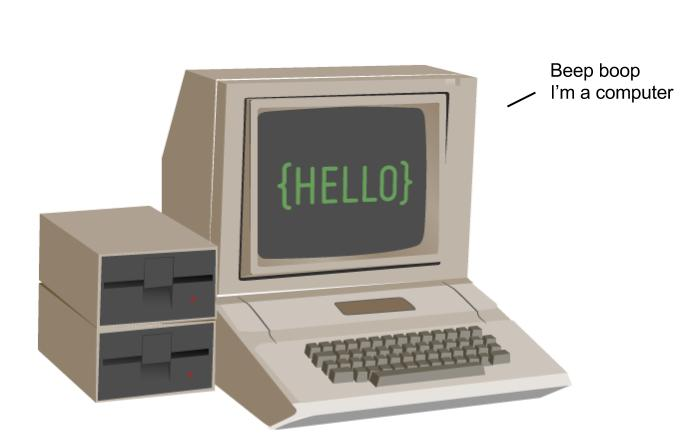
\includegraphics[width=0.5\textwidth]{beepboop.jpg}
  \end{center}
\end{frame}

\begin{frame}
  \frametitle{Binary}
  The mathematics of binary are actually just as simple as 
  with decimal, we just aren't used to seeing them.
  In decimal, if you add a 1 to a 9 it \textbf{carrys over} 
  to the next digit. In binary when you add a 1 to a 1 
  it \textbf{carrys over}.\\
  \begin{center}
    \begin{tabular}{r}
      01\\
      +01\\
      \hline
      10\\
    \end{tabular}
  \end{center}
  \begin{center}
    \begin{tabular}{r}
      011\\
      +001\\
      \hline
      100\\
    \end{tabular}
  \end{center}
\end{frame}

\begin{frame}
  \frametitle{Binary}
  In decimal, each digit of a number means 
  that number can represenent another power of 10.
  Thus, a 3 digit number can represent $10^3$ worth
  of numbers (0, 1, 2, 3, ...998, 999).\\
  \vspace{12pt}
  Similarly, if a binary number has $n$ digits, it can
  represent $2^n$ numbers. So a 3 digit binary number
  can represent $2^3 = 8$ numbers (0, 1, 2, 3, 4, 5, 6, 7).\\
  Don't believe me? See for yourself:\\
  \begin{center}
    \begin{tabular}{ll}
      0 & 000\\
      1 & 001\\
      2 & 010\\
      3 & 011\\
      4 & 100\\
      5 & 101\\
      6 & 110\\
      7 & 111\\
    \end{tabular}
  \end{center}
\end{frame}

\begin{frame}
  \frametitle{Bits and bytes}
  In binary, a single digit is called a \textbf{bit}.\\
  As we just saw, more bits means we can store more information.\\
  Eight \textbf{bits} are called a \textbf{byte}.\\
  A thousand \textbf{bytes} are called a \textbf{kilobyte}, and so on.
\end{frame}

\begin{frame}[fragile]
  \frametitle{More Types}
  So far you have learned about integers (\textbf{int}) and floating point numbers (\textbf{floats}).
  Here is a list of all of the types available in the C language:
  \begin{tabular}{ll}
      void & no type. Often this means no variable.\\
      char & character\\
      short & integer\\
      int  & integer\\
      long & integer\\
      float & floating point number\\
      double & floating point number. It is twice the size of a float\\
      long double & floating point number. It is even bigger\\
  \end{tabular}
\end{frame}

\begin{frame}[fragile]
  \frametitle{Emacs in the background}
  We are about to write a program called sizeof.c. However, when you open
  it in emacs try putting a ``\&'' at the end.
  \begin{lstlisting}[style=custombash]
    emacs sizeof.c &
  \end{lstlisting}
  This will run emacs in the background and give you access to the terminal
  at the same time. This way you can compile while emacs is still open :).
\end{frame}

\begin{frame}[fragile,allowframebreaks]
  \frametitle{sizeof.c}
  In order to figure out the size of these types, we can use the funciton \textbf{sizeof()}.\\
  It gives us the size in \textbf{bytes} of the variable passed in.
  \lstinputlisting[style=customc]{sizeof.c}
\end{frame}

\begin{frame}
  \frametitle{Why not use larger variables?}
  You might as yourself ``If a long can hold more than an int, and a double can hold more than a float, why not always use those larger types?''\\
  That's a good question, and the answer is that 
  it depends on the program you are writing.\\
  In general though, using the smallest type possible 
  for a program will allow the program to run faster,
  while using larger types might allow higher precision.
\end{frame}

\begin{frame}
  \frametitle{Loops}
  What if you wanted to do a single action over an over?\\
  For instance, what if you wanted to take a variable that
  was equal to 0 and add 2 to it one hundred times?\\
  \begin{center}
    \begin{equation*}
      x = \sum_{i=0}^{100}2
    \end{equation*}
  \end{center}
  Instead of writing $x = x +2$ one hundred times, you can use \textbf{loops}.
\end{frame}

\begin{frame}[fragile]
  \frametitle{For loops}
  Today we will learn to use \textbf{for} loops.\\
  The structure of a for loop is very simple:
  \begin{lstlisting}[style=customc]
    ... // before the for loop
    for(start; condition; iteration){
      ... // inside the for loop block is repeated
    }
    ... //after the for loop
  \end{lstlisting}
  \textit{Start} gives some starting point.\\ \textit{Condition} gives some
  true/false statement that tells the loop when to end (e.g. $x<10$ or $i==9$).\\
  \textit{Iteration} tells the loop how to count each step (e.g. $i=i+1$ or 
  $x = x - 0.2$ or $y = 2y$).
\end{frame}

\begin{frame}[fragile]
  \frametitle{For loops}
  For our previous example, this would look like:
  \begin{lstlisting}[style=customc]
    int i;
    int x = 0;
    for( i=0; i<100; i=i+1){
      x = x + 2;
    }
  \end{lstlisting}
  The loop performed 100 iterations or steps (0, 1, 2, ...98, 99).\\
  After each iteration a 2 was added to $x$.\\
  Therefore, after the loop $x=200$.
\end{frame}

\begin{frame}[fragile]
  \frametitle{blastoff.c}
  Here is a simple program that uses a loop to count down from 10 
  before a rocket blasts off.
  \lstinputlisting[style=customc]{blastoff.c}
\end{frame}

\begin{frame}
  \frametitle{HW 3 - Quadratic equation due in 2 weeks}
  A quadratic function has the form:
  \begin{equation*}
    y(x) = ax^2 + bx + c
  \end{equation*}
  This function has two or fewer roots, or locations 
  where it crosses the x-axis.\\
  The equation to find these roots is called the quadratic equation.
  \begin{equation*}
    x_\pm = \frac{-b\pm\sqrt{b^2-4ac}}{2a}
  \end{equation*}
  Take in the coefficients $a$, $b$ and $c$ from the user and use them
  to calculate the roots from the quadratic equation.\\
  Make sure to account for the cases when there are no roots!!
\end{frame}

\begin{frame}[allowframebreaks]
  \frametitle{In class assignments}
  Today there are two in class assignments
  \vspace{0.75in}
  \begin{enumerate}
  \item Figure out on paper what the largest positive and negative \textbf{short},
    \textbf{int}, and \textbf{long} variables are. Write a program that prints these
    values. Note: remember that one bit is used for the positive/negative sign,
    so even though a \textbf{short} is 2 bytes (16 bits) it is really 15 bits!!!
    \newpage
  \item Write a program that prints out a dozen x's to the screen.\\
    \begin{center}
      xxxxxxxxxxxx
    \end{center}
    Once that is complete, modify this program so that it prints a dozen lines each
    with a dozen x's.
    \begin{center}
      xxxxxxxxxxxx\\
      xxxxxxxxxxxx\\
      xxxxxxxxxxxx\\
      xxxxxxxxxxxx\\
      xxxxxxxxxxxx\\
      xxxxxxxxxxxx\\
      xxxxxxxxxxxx\\
      xxxxxxxxxxxx\\
      xxxxxxxxxxxx\\
      xxxxxxxxxxxx\\
      xxxxxxxxxxxx\\
      xxxxxxxxxxxx
    \end{center}
  \end{enumerate}
\end{frame}

\begin{frame}
  \frametitle{Next time}
  \begin{itemize}
    \item Character strings
    \item Arrays
  \end{itemize}
\end{frame}

\begin{frame}[fragile]
  \frametitle{Size of types}
  For reference, here are all of the sizes of the types
  \begin{tabular}{ll}
      void & no type. Often this means no variable.\\
      char & character, usually 1 byte (8 bits)\\
      short & integer, 2 bytes (16 bits)\\
      int  & integer, 4 bytes (32 bits)\\
      long & integer, 8 bytes (64 bits)\\
      float & floating point number of 4 bytes\\
      double & floating point number usually 8 bytes.\\
      long double & floating point number usually 16 bytes\\
  \end{tabular}
\end{frame}



\end{document}